\hspace*{\fill}\panel{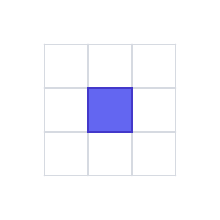
\begin{tikzpicture}[x=1bp, y=1bp]\path[use as bounding box] (0,0) rectangle (59.25,59.25);\clip (0,0) rectangle (59.25,59.25);
\path[draw={rgb,255:red,214;green,218;blue,225}, line width=0.60bp, line cap=round, line join=round] (6.00,6.00) -- (6.00,53.25);
\path[draw={rgb,255:red,214;green,218;blue,225}, line width=0.60bp, line cap=round, line join=round] (21.75,6.00) -- (21.75,53.25);
\path[draw={rgb,255:red,214;green,218;blue,225}, line width=0.60bp, line cap=round, line join=round] (37.50,6.00) -- (37.50,53.25);
\path[draw={rgb,255:red,214;green,218;blue,225}, line width=0.60bp, line cap=round, line join=round] (53.25,6.00) -- (53.25,53.25);
\path[draw={rgb,255:red,214;green,218;blue,225}, line width=0.60bp, line cap=round, line join=round] (6.00,6.00) -- (53.25,6.00);
\path[draw={rgb,255:red,214;green,218;blue,225}, line width=0.60bp, line cap=round, line join=round] (6.00,21.75) -- (53.25,21.75);
\path[draw={rgb,255:red,214;green,218;blue,225}, line width=0.60bp, line cap=round, line join=round] (6.00,37.50) -- (53.25,37.50);
\path[draw={rgb,255:red,214;green,218;blue,225}, line width=0.60bp, line cap=round, line join=round] (6.00,53.25) -- (53.25,53.25);
\path[draw={rgb,255:red,67;green,56;blue,202}, line width=0.60bp, fill={rgb,255:red,99;green,102;blue,241}] (21.75,21.75) rectangle (37.50,37.50);
\end{tikzpicture}}{one cell}\hfill\panel{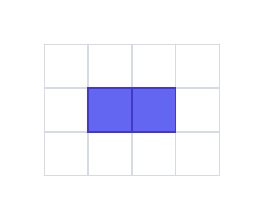
\begin{tikzpicture}[x=1bp, y=1bp]\path[use as bounding box] (0,0) rectangle (75.00,59.25);\clip (0,0) rectangle (75.00,59.25);
\path[draw={rgb,255:red,214;green,218;blue,225}, line width=0.60bp, line cap=round, line join=round] (6.00,6.00) -- (6.00,53.25);
\path[draw={rgb,255:red,214;green,218;blue,225}, line width=0.60bp, line cap=round, line join=round] (21.75,6.00) -- (21.75,53.25);
\path[draw={rgb,255:red,214;green,218;blue,225}, line width=0.60bp, line cap=round, line join=round] (37.50,6.00) -- (37.50,53.25);
\path[draw={rgb,255:red,214;green,218;blue,225}, line width=0.60bp, line cap=round, line join=round] (53.25,6.00) -- (53.25,53.25);
\path[draw={rgb,255:red,214;green,218;blue,225}, line width=0.60bp, line cap=round, line join=round] (69.00,6.00) -- (69.00,53.25);
\path[draw={rgb,255:red,214;green,218;blue,225}, line width=0.60bp, line cap=round, line join=round] (6.00,6.00) -- (69.00,6.00);
\path[draw={rgb,255:red,214;green,218;blue,225}, line width=0.60bp, line cap=round, line join=round] (6.00,21.75) -- (69.00,21.75);
\path[draw={rgb,255:red,214;green,218;blue,225}, line width=0.60bp, line cap=round, line join=round] (6.00,37.50) -- (69.00,37.50);
\path[draw={rgb,255:red,214;green,218;blue,225}, line width=0.60bp, line cap=round, line join=round] (6.00,53.25) -- (69.00,53.25);
\path[draw={rgb,255:red,67;green,56;blue,202}, line width=0.60bp, fill={rgb,255:red,99;green,102;blue,241}] (21.75,21.75) rectangle (37.50,37.50);
\path[draw={rgb,255:red,67;green,56;blue,202}, line width=0.60bp, fill={rgb,255:red,99;green,102;blue,241}] (37.50,21.75) rectangle (53.25,37.50);
\end{tikzpicture}}{domino}\hfill\panel{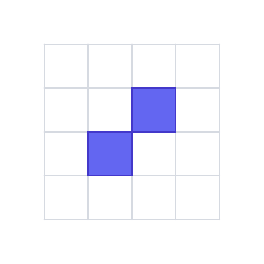
\begin{tikzpicture}[x=1bp, y=1bp]\path[use as bounding box] (0,0) rectangle (75.00,75.00);\clip (0,0) rectangle (75.00,75.00);
\path[draw={rgb,255:red,214;green,218;blue,225}, line width=0.60bp, line cap=round, line join=round] (6.00,6.00) -- (6.00,69.00);
\path[draw={rgb,255:red,214;green,218;blue,225}, line width=0.60bp, line cap=round, line join=round] (21.75,6.00) -- (21.75,69.00);
\path[draw={rgb,255:red,214;green,218;blue,225}, line width=0.60bp, line cap=round, line join=round] (37.50,6.00) -- (37.50,69.00);
\path[draw={rgb,255:red,214;green,218;blue,225}, line width=0.60bp, line cap=round, line join=round] (53.25,6.00) -- (53.25,69.00);
\path[draw={rgb,255:red,214;green,218;blue,225}, line width=0.60bp, line cap=round, line join=round] (69.00,6.00) -- (69.00,69.00);
\path[draw={rgb,255:red,214;green,218;blue,225}, line width=0.60bp, line cap=round, line join=round] (6.00,6.00) -- (69.00,6.00);
\path[draw={rgb,255:red,214;green,218;blue,225}, line width=0.60bp, line cap=round, line join=round] (6.00,21.75) -- (69.00,21.75);
\path[draw={rgb,255:red,214;green,218;blue,225}, line width=0.60bp, line cap=round, line join=round] (6.00,37.50) -- (69.00,37.50);
\path[draw={rgb,255:red,214;green,218;blue,225}, line width=0.60bp, line cap=round, line join=round] (6.00,53.25) -- (69.00,53.25);
\path[draw={rgb,255:red,214;green,218;blue,225}, line width=0.60bp, line cap=round, line join=round] (6.00,69.00) -- (69.00,69.00);
\path[draw={rgb,255:red,67;green,56;blue,202}, line width=0.60bp, fill={rgb,255:red,99;green,102;blue,241}] (21.75,21.75) rectangle (37.50,37.50);
\path[draw={rgb,255:red,67;green,56;blue,202}, line width=0.60bp, fill={rgb,255:red,99;green,102;blue,241}] (37.50,37.50) rectangle (53.25,53.25);
\end{tikzpicture}}{diagonal pair}\hfill\panel{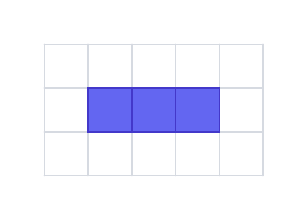
\begin{tikzpicture}[x=1bp, y=1bp]\path[use as bounding box] (0,0) rectangle (90.75,59.25);\clip (0,0) rectangle (90.75,59.25);
\path[draw={rgb,255:red,214;green,218;blue,225}, line width=0.60bp, line cap=round, line join=round] (6.00,6.00) -- (6.00,53.25);
\path[draw={rgb,255:red,214;green,218;blue,225}, line width=0.60bp, line cap=round, line join=round] (21.75,6.00) -- (21.75,53.25);
\path[draw={rgb,255:red,214;green,218;blue,225}, line width=0.60bp, line cap=round, line join=round] (37.50,6.00) -- (37.50,53.25);
\path[draw={rgb,255:red,214;green,218;blue,225}, line width=0.60bp, line cap=round, line join=round] (53.25,6.00) -- (53.25,53.25);
\path[draw={rgb,255:red,214;green,218;blue,225}, line width=0.60bp, line cap=round, line join=round] (69.00,6.00) -- (69.00,53.25);
\path[draw={rgb,255:red,214;green,218;blue,225}, line width=0.60bp, line cap=round, line join=round] (84.75,6.00) -- (84.75,53.25);
\path[draw={rgb,255:red,214;green,218;blue,225}, line width=0.60bp, line cap=round, line join=round] (6.00,6.00) -- (84.75,6.00);
\path[draw={rgb,255:red,214;green,218;blue,225}, line width=0.60bp, line cap=round, line join=round] (6.00,21.75) -- (84.75,21.75);
\path[draw={rgb,255:red,214;green,218;blue,225}, line width=0.60bp, line cap=round, line join=round] (6.00,37.50) -- (84.75,37.50);
\path[draw={rgb,255:red,214;green,218;blue,225}, line width=0.60bp, line cap=round, line join=round] (6.00,53.25) -- (84.75,53.25);
\path[draw={rgb,255:red,67;green,56;blue,202}, line width=0.60bp, fill={rgb,255:red,99;green,102;blue,241}] (21.75,21.75) rectangle (37.50,37.50);
\path[draw={rgb,255:red,67;green,56;blue,202}, line width=0.60bp, fill={rgb,255:red,99;green,102;blue,241}] (37.50,21.75) rectangle (53.25,37.50);
\path[draw={rgb,255:red,67;green,56;blue,202}, line width=0.60bp, fill={rgb,255:red,99;green,102;blue,241}] (53.25,21.75) rectangle (69.00,37.50);
\end{tikzpicture}}{line of 3}\hfill\panel{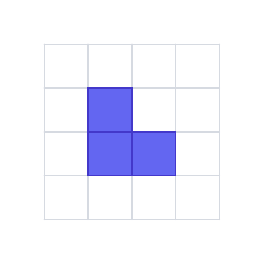
\begin{tikzpicture}[x=1bp, y=1bp]\path[use as bounding box] (0,0) rectangle (75.00,75.00);\clip (0,0) rectangle (75.00,75.00);
\path[draw={rgb,255:red,214;green,218;blue,225}, line width=0.60bp, line cap=round, line join=round] (6.00,6.00) -- (6.00,69.00);
\path[draw={rgb,255:red,214;green,218;blue,225}, line width=0.60bp, line cap=round, line join=round] (21.75,6.00) -- (21.75,69.00);
\path[draw={rgb,255:red,214;green,218;blue,225}, line width=0.60bp, line cap=round, line join=round] (37.50,6.00) -- (37.50,69.00);
\path[draw={rgb,255:red,214;green,218;blue,225}, line width=0.60bp, line cap=round, line join=round] (53.25,6.00) -- (53.25,69.00);
\path[draw={rgb,255:red,214;green,218;blue,225}, line width=0.60bp, line cap=round, line join=round] (69.00,6.00) -- (69.00,69.00);
\path[draw={rgb,255:red,214;green,218;blue,225}, line width=0.60bp, line cap=round, line join=round] (6.00,6.00) -- (69.00,6.00);
\path[draw={rgb,255:red,214;green,218;blue,225}, line width=0.60bp, line cap=round, line join=round] (6.00,21.75) -- (69.00,21.75);
\path[draw={rgb,255:red,214;green,218;blue,225}, line width=0.60bp, line cap=round, line join=round] (6.00,37.50) -- (69.00,37.50);
\path[draw={rgb,255:red,214;green,218;blue,225}, line width=0.60bp, line cap=round, line join=round] (6.00,53.25) -- (69.00,53.25);
\path[draw={rgb,255:red,214;green,218;blue,225}, line width=0.60bp, line cap=round, line join=round] (6.00,69.00) -- (69.00,69.00);
\path[draw={rgb,255:red,67;green,56;blue,202}, line width=0.60bp, fill={rgb,255:red,99;green,102;blue,241}] (21.75,21.75) rectangle (37.50,37.50);
\path[draw={rgb,255:red,67;green,56;blue,202}, line width=0.60bp, fill={rgb,255:red,99;green,102;blue,241}] (37.50,21.75) rectangle (53.25,37.50);
\path[draw={rgb,255:red,67;green,56;blue,202}, line width=0.60bp, fill={rgb,255:red,99;green,102;blue,241}] (21.75,37.50) rectangle (37.50,53.25);
\end{tikzpicture}}{L of 3}\hspace*{\fill}\par\medskip
\hspace*{\fill}\panel{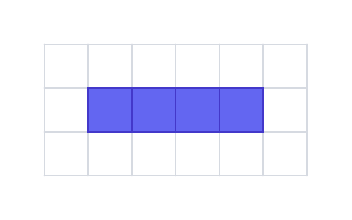
\begin{tikzpicture}[x=1bp, y=1bp]\path[use as bounding box] (0,0) rectangle (106.50,59.25);\clip (0,0) rectangle (106.50,59.25);
\path[draw={rgb,255:red,214;green,218;blue,225}, line width=0.60bp, line cap=round, line join=round] (6.00,6.00) -- (6.00,53.25);
\path[draw={rgb,255:red,214;green,218;blue,225}, line width=0.60bp, line cap=round, line join=round] (21.75,6.00) -- (21.75,53.25);
\path[draw={rgb,255:red,214;green,218;blue,225}, line width=0.60bp, line cap=round, line join=round] (37.50,6.00) -- (37.50,53.25);
\path[draw={rgb,255:red,214;green,218;blue,225}, line width=0.60bp, line cap=round, line join=round] (53.25,6.00) -- (53.25,53.25);
\path[draw={rgb,255:red,214;green,218;blue,225}, line width=0.60bp, line cap=round, line join=round] (69.00,6.00) -- (69.00,53.25);
\path[draw={rgb,255:red,214;green,218;blue,225}, line width=0.60bp, line cap=round, line join=round] (84.75,6.00) -- (84.75,53.25);
\path[draw={rgb,255:red,214;green,218;blue,225}, line width=0.60bp, line cap=round, line join=round] (100.50,6.00) -- (100.50,53.25);
\path[draw={rgb,255:red,214;green,218;blue,225}, line width=0.60bp, line cap=round, line join=round] (6.00,6.00) -- (100.50,6.00);
\path[draw={rgb,255:red,214;green,218;blue,225}, line width=0.60bp, line cap=round, line join=round] (6.00,21.75) -- (100.50,21.75);
\path[draw={rgb,255:red,214;green,218;blue,225}, line width=0.60bp, line cap=round, line join=round] (6.00,37.50) -- (100.50,37.50);
\path[draw={rgb,255:red,214;green,218;blue,225}, line width=0.60bp, line cap=round, line join=round] (6.00,53.25) -- (100.50,53.25);
\path[draw={rgb,255:red,67;green,56;blue,202}, line width=0.60bp, fill={rgb,255:red,99;green,102;blue,241}] (21.75,21.75) rectangle (37.50,37.50);
\path[draw={rgb,255:red,67;green,56;blue,202}, line width=0.60bp, fill={rgb,255:red,99;green,102;blue,241}] (37.50,21.75) rectangle (53.25,37.50);
\path[draw={rgb,255:red,67;green,56;blue,202}, line width=0.60bp, fill={rgb,255:red,99;green,102;blue,241}] (53.25,21.75) rectangle (69.00,37.50);
\path[draw={rgb,255:red,67;green,56;blue,202}, line width=0.60bp, fill={rgb,255:red,99;green,102;blue,241}] (69.00,21.75) rectangle (84.75,37.50);
\end{tikzpicture}}{I shape}\hfill\panel{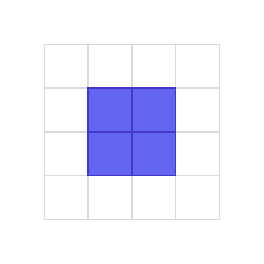
\begin{tikzpicture}[x=1bp, y=1bp]\path[use as bounding box] (0,0) rectangle (75.00,75.00);\clip (0,0) rectangle (75.00,75.00);
\path[draw={rgb,255:red,214;green,218;blue,225}, line width=0.60bp, line cap=round, line join=round] (6.00,6.00) -- (6.00,69.00);
\path[draw={rgb,255:red,214;green,218;blue,225}, line width=0.60bp, line cap=round, line join=round] (21.75,6.00) -- (21.75,69.00);
\path[draw={rgb,255:red,214;green,218;blue,225}, line width=0.60bp, line cap=round, line join=round] (37.50,6.00) -- (37.50,69.00);
\path[draw={rgb,255:red,214;green,218;blue,225}, line width=0.60bp, line cap=round, line join=round] (53.25,6.00) -- (53.25,69.00);
\path[draw={rgb,255:red,214;green,218;blue,225}, line width=0.60bp, line cap=round, line join=round] (69.00,6.00) -- (69.00,69.00);
\path[draw={rgb,255:red,214;green,218;blue,225}, line width=0.60bp, line cap=round, line join=round] (6.00,6.00) -- (69.00,6.00);
\path[draw={rgb,255:red,214;green,218;blue,225}, line width=0.60bp, line cap=round, line join=round] (6.00,21.75) -- (69.00,21.75);
\path[draw={rgb,255:red,214;green,218;blue,225}, line width=0.60bp, line cap=round, line join=round] (6.00,37.50) -- (69.00,37.50);
\path[draw={rgb,255:red,214;green,218;blue,225}, line width=0.60bp, line cap=round, line join=round] (6.00,53.25) -- (69.00,53.25);
\path[draw={rgb,255:red,214;green,218;blue,225}, line width=0.60bp, line cap=round, line join=round] (6.00,69.00) -- (69.00,69.00);
\path[draw={rgb,255:red,67;green,56;blue,202}, line width=0.60bp, fill={rgb,255:red,99;green,102;blue,241}] (21.75,21.75) rectangle (37.50,37.50);
\path[draw={rgb,255:red,67;green,56;blue,202}, line width=0.60bp, fill={rgb,255:red,99;green,102;blue,241}] (37.50,21.75) rectangle (53.25,37.50);
\path[draw={rgb,255:red,67;green,56;blue,202}, line width=0.60bp, fill={rgb,255:red,99;green,102;blue,241}] (21.75,37.50) rectangle (37.50,53.25);
\path[draw={rgb,255:red,67;green,56;blue,202}, line width=0.60bp, fill={rgb,255:red,99;green,102;blue,241}] (37.50,37.50) rectangle (53.25,53.25);
\end{tikzpicture}}{O shape}\hfill\panel{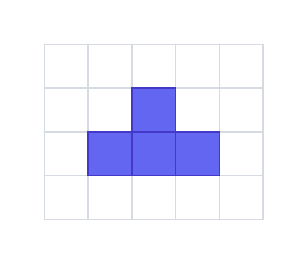
\begin{tikzpicture}[x=1bp, y=1bp]\path[use as bounding box] (0,0) rectangle (90.75,75.00);\clip (0,0) rectangle (90.75,75.00);
\path[draw={rgb,255:red,214;green,218;blue,225}, line width=0.60bp, line cap=round, line join=round] (6.00,6.00) -- (6.00,69.00);
\path[draw={rgb,255:red,214;green,218;blue,225}, line width=0.60bp, line cap=round, line join=round] (21.75,6.00) -- (21.75,69.00);
\path[draw={rgb,255:red,214;green,218;blue,225}, line width=0.60bp, line cap=round, line join=round] (37.50,6.00) -- (37.50,69.00);
\path[draw={rgb,255:red,214;green,218;blue,225}, line width=0.60bp, line cap=round, line join=round] (53.25,6.00) -- (53.25,69.00);
\path[draw={rgb,255:red,214;green,218;blue,225}, line width=0.60bp, line cap=round, line join=round] (69.00,6.00) -- (69.00,69.00);
\path[draw={rgb,255:red,214;green,218;blue,225}, line width=0.60bp, line cap=round, line join=round] (84.75,6.00) -- (84.75,69.00);
\path[draw={rgb,255:red,214;green,218;blue,225}, line width=0.60bp, line cap=round, line join=round] (6.00,6.00) -- (84.75,6.00);
\path[draw={rgb,255:red,214;green,218;blue,225}, line width=0.60bp, line cap=round, line join=round] (6.00,21.75) -- (84.75,21.75);
\path[draw={rgb,255:red,214;green,218;blue,225}, line width=0.60bp, line cap=round, line join=round] (6.00,37.50) -- (84.75,37.50);
\path[draw={rgb,255:red,214;green,218;blue,225}, line width=0.60bp, line cap=round, line join=round] (6.00,53.25) -- (84.75,53.25);
\path[draw={rgb,255:red,214;green,218;blue,225}, line width=0.60bp, line cap=round, line join=round] (6.00,69.00) -- (84.75,69.00);
\path[draw={rgb,255:red,67;green,56;blue,202}, line width=0.60bp, fill={rgb,255:red,99;green,102;blue,241}] (21.75,21.75) rectangle (37.50,37.50);
\path[draw={rgb,255:red,67;green,56;blue,202}, line width=0.60bp, fill={rgb,255:red,99;green,102;blue,241}] (37.50,21.75) rectangle (53.25,37.50);
\path[draw={rgb,255:red,67;green,56;blue,202}, line width=0.60bp, fill={rgb,255:red,99;green,102;blue,241}] (53.25,21.75) rectangle (69.00,37.50);
\path[draw={rgb,255:red,67;green,56;blue,202}, line width=0.60bp, fill={rgb,255:red,99;green,102;blue,241}] (37.50,37.50) rectangle (53.25,53.25);
\end{tikzpicture}}{T shape}\hfill\panel{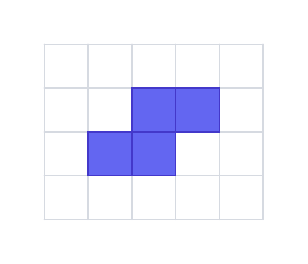
\begin{tikzpicture}[x=1bp, y=1bp]\path[use as bounding box] (0,0) rectangle (90.75,75.00);\clip (0,0) rectangle (90.75,75.00);
\path[draw={rgb,255:red,214;green,218;blue,225}, line width=0.60bp, line cap=round, line join=round] (6.00,6.00) -- (6.00,69.00);
\path[draw={rgb,255:red,214;green,218;blue,225}, line width=0.60bp, line cap=round, line join=round] (21.75,6.00) -- (21.75,69.00);
\path[draw={rgb,255:red,214;green,218;blue,225}, line width=0.60bp, line cap=round, line join=round] (37.50,6.00) -- (37.50,69.00);
\path[draw={rgb,255:red,214;green,218;blue,225}, line width=0.60bp, line cap=round, line join=round] (53.25,6.00) -- (53.25,69.00);
\path[draw={rgb,255:red,214;green,218;blue,225}, line width=0.60bp, line cap=round, line join=round] (69.00,6.00) -- (69.00,69.00);
\path[draw={rgb,255:red,214;green,218;blue,225}, line width=0.60bp, line cap=round, line join=round] (84.75,6.00) -- (84.75,69.00);
\path[draw={rgb,255:red,214;green,218;blue,225}, line width=0.60bp, line cap=round, line join=round] (6.00,6.00) -- (84.75,6.00);
\path[draw={rgb,255:red,214;green,218;blue,225}, line width=0.60bp, line cap=round, line join=round] (6.00,21.75) -- (84.75,21.75);
\path[draw={rgb,255:red,214;green,218;blue,225}, line width=0.60bp, line cap=round, line join=round] (6.00,37.50) -- (84.75,37.50);
\path[draw={rgb,255:red,214;green,218;blue,225}, line width=0.60bp, line cap=round, line join=round] (6.00,53.25) -- (84.75,53.25);
\path[draw={rgb,255:red,214;green,218;blue,225}, line width=0.60bp, line cap=round, line join=round] (6.00,69.00) -- (84.75,69.00);
\path[draw={rgb,255:red,67;green,56;blue,202}, line width=0.60bp, fill={rgb,255:red,99;green,102;blue,241}] (21.75,21.75) rectangle (37.50,37.50);
\path[draw={rgb,255:red,67;green,56;blue,202}, line width=0.60bp, fill={rgb,255:red,99;green,102;blue,241}] (37.50,21.75) rectangle (53.25,37.50);
\path[draw={rgb,255:red,67;green,56;blue,202}, line width=0.60bp, fill={rgb,255:red,99;green,102;blue,241}] (37.50,37.50) rectangle (53.25,53.25);
\path[draw={rgb,255:red,67;green,56;blue,202}, line width=0.60bp, fill={rgb,255:red,99;green,102;blue,241}] (53.25,37.50) rectangle (69.00,53.25);
\end{tikzpicture}}{S shape}\hfill\panel{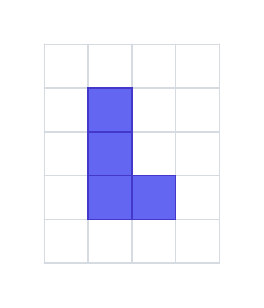
\begin{tikzpicture}[x=1bp, y=1bp]\path[use as bounding box] (0,0) rectangle (75.00,90.75);\clip (0,0) rectangle (75.00,90.75);
\path[draw={rgb,255:red,214;green,218;blue,225}, line width=0.60bp, line cap=round, line join=round] (6.00,6.00) -- (6.00,84.75);
\path[draw={rgb,255:red,214;green,218;blue,225}, line width=0.60bp, line cap=round, line join=round] (21.75,6.00) -- (21.75,84.75);
\path[draw={rgb,255:red,214;green,218;blue,225}, line width=0.60bp, line cap=round, line join=round] (37.50,6.00) -- (37.50,84.75);
\path[draw={rgb,255:red,214;green,218;blue,225}, line width=0.60bp, line cap=round, line join=round] (53.25,6.00) -- (53.25,84.75);
\path[draw={rgb,255:red,214;green,218;blue,225}, line width=0.60bp, line cap=round, line join=round] (69.00,6.00) -- (69.00,84.75);
\path[draw={rgb,255:red,214;green,218;blue,225}, line width=0.60bp, line cap=round, line join=round] (6.00,6.00) -- (69.00,6.00);
\path[draw={rgb,255:red,214;green,218;blue,225}, line width=0.60bp, line cap=round, line join=round] (6.00,21.75) -- (69.00,21.75);
\path[draw={rgb,255:red,214;green,218;blue,225}, line width=0.60bp, line cap=round, line join=round] (6.00,37.50) -- (69.00,37.50);
\path[draw={rgb,255:red,214;green,218;blue,225}, line width=0.60bp, line cap=round, line join=round] (6.00,53.25) -- (69.00,53.25);
\path[draw={rgb,255:red,214;green,218;blue,225}, line width=0.60bp, line cap=round, line join=round] (6.00,69.00) -- (69.00,69.00);
\path[draw={rgb,255:red,214;green,218;blue,225}, line width=0.60bp, line cap=round, line join=round] (6.00,84.75) -- (69.00,84.75);
\path[draw={rgb,255:red,67;green,56;blue,202}, line width=0.60bp, fill={rgb,255:red,99;green,102;blue,241}] (21.75,21.75) rectangle (37.50,37.50);
\path[draw={rgb,255:red,67;green,56;blue,202}, line width=0.60bp, fill={rgb,255:red,99;green,102;blue,241}] (21.75,37.50) rectangle (37.50,53.25);
\path[draw={rgb,255:red,67;green,56;blue,202}, line width=0.60bp, fill={rgb,255:red,99;green,102;blue,241}] (21.75,53.25) rectangle (37.50,69.00);
\path[draw={rgb,255:red,67;green,56;blue,202}, line width=0.60bp, fill={rgb,255:red,99;green,102;blue,241}] (37.50,21.75) rectangle (53.25,37.50);
\end{tikzpicture}}{L shape}\hspace*{\fill}
